% TEMPO-BIAS report — compiles with LuaLaTeX or XeLaTeX
\documentclass[11pt]{article}

\usepackage[review]{acl}
\usepackage{microtype}
\usepackage[english,bidi=default]{babel}
% Latin Modern Roman (bundled with TeX Live). For TeXGyre Termes X, use: \babelfont{rm}{TeXGyreTermesX}
\babelfont{rm}{Latin Modern Roman}

\usepackage{graphicx}
\usepackage{amsmath}
\usepackage{booktabs}

\title{Political Bias and Temporal Dynamics in Large Language Models}

\author{Ran Lu \\
  Université Paris-Saclay \\
  \texttt{ran.lu@universite-paris-saclay.fr} \\\And
  Hasti Hosseinpour \\
  Université Paris-Saclay \\
  \texttt{hasti.hosseinpour@universite-paris-saclay.fr} \\\And
  Abderrahmane Moujar \\
  Université Paris-Saclay \\
  \texttt{abderrahmane.moujar@universite-paris-saclay.fr} \\\And
  Oloruntobi Olutola \\
  Université Paris-Saclay \\
  \texttt{oloruntobi.olutola@universite-paris-saclay.fr}}

\begin{document}
\maketitle

\begin{abstract}
Large language models (LLMs) increasingly mediate how users access and interpret political information, yet most studies of political bias treat models as static. We study bias as a \emph{temporal} phenomenon using Prediction Inconsistency (IC) and sentiment label distributions on target-oriented classification. We evaluate two families---OpenAI ChatGPT (gpt-3.5-turbo through gpt-4o) and Meta Llama~3.2 (Base and Instruct, 1B--11B)---on fixed entities and templates. For ChatGPT, IC rises from near zero (gpt-3.5-turbo) to $\approx$0.67 (gpt-4) and plateaus at $\approx$0.61 for later variants; labels shift from 100\% positive to a mix of positive and UNKNOWN. For Llama, IC is lower (0.005--0.178); instruction tuning sharply reduces IC for 1B and yields minimal inconsistency for the 11B vision model. We show that political bias, as captured by IC and label distribution, evolves with model family, version, and alignment, and argue for longitudinal evaluation in bias research.
\end{abstract}

\section{Introduction}

Large language models have become central intermediaries in how people access, interpret, and evaluate political information. Their use in summarization, question answering, and sentiment analysis gives them substantial influence over public discourse. A growing body of work demonstrates that LLMs are not ideologically neutral: political tendencies emerge from training data, architecture, and alignment \citep{santurkar2023,buyl2026,hartmann2023,bang2024}. When models systematically favor or disfavor certain actors or viewpoints, they can function as implicit instruments of political influence.

Most prior work evaluates political bias at a single point in time. This static view is increasingly inadequate. Model families such as LLaMA and GPT evolve rapidly; training corpora, safety data, and alignment procedures change across generations \citep{touvron2023,dubey2024}. Such interventions may affect not only safety and factuality but also political framing and sentiment. We therefore study political bias through a \emph{temporal} lens: how does it change across model generations and alignment stages?

We adopt the framework of \citet{elbouanani2025}, who quantify bias via Prediction Inconsistency (IC)---the instability of sentiment predictions when the target political entity is swapped in a sentence. We extend this to a longitudinal setting and evaluate two families: OpenAI ChatGPT (five versions from gpt-3.5-turbo to gpt-4o) and Meta Llama~3.2 (Base and Instruct, including 1B, 3B, and 11B vision). Our research questions are: (1) How does IC evolve across model versions? (2) How does alignment (Base vs.\ Instruct) affect IC and sentiment label distribution? (3) How do these patterns differ across families?

Our contributions are: (i) a temporal view of political bias in LLMs; (ii) longitudinal IC and label-distribution results for ChatGPT and Llama on the same task; and (iii) evidence that the effect of alignment on bias is size- and family-dependent.

\section{Related Work}

Political bias in LLMs has been studied along several axes. Early work mapped model outputs onto ideological frameworks \citep{santurkar2023,hartmann2023}. Later studies distinguished explicit stance from framing and lexical polarity \citep{bang2024} and operationalized bias via target-oriented sentiment classification \citep{wang2025,chen2024}. \citet{elbouanani2025} introduce Prediction Inconsistency (IC) as the entropy of predicted labels across entity substitutions; we adopt this metric and extend it to a temporal setting.

Temporal drift in LLM behavior and bias is well documented \citep{zhu2024,buyl2026}. Technical reports on LLaMA describe substantial changes in safety data and alignment across generations \citep{touvron2023,dubey2024}; comparative evaluations show that newer models handle politically nuanced content differently \citep{crum2024}. Mitigation and alignment can alter political nuance \citep{banko2025,bonaldi2024}. We contribute a direct, longitudinal comparison of IC and label distributions across ChatGPT and Llama under controlled prompts and entities.

\section{Methodology}

We follow \citet{elbouanani2025}. \textbf{Data.} We use 250 political entities from major regions and 60 sentence templates (positive, neutral, negative). Entity names are substituted into templates; the only varying factor per prompt is the entity. \textbf{Task.} Target-oriented sentiment classification (TSC): models predict one of \{\text{positive}, \text{neutral}, \text{negative}\}. \textbf{Metric.} Prediction Inconsistency (IC). For each template $s$, we obtain a distribution over labels across entities:
$P(l|s) = |\{e \in E : \text{pred}(s,e)=l\}|/|E|$. The entropy $H(s) = -\sum_l P(l|s)\log P(l|s)$ measures inconsistency for that template; we report the average over templates: $\text{IC} = \frac{1}{m}\sum_i H(s_i)$. IC = 0 corresponds to perfectly consistent (unbiased) predictions.

\textbf{Setup.} We use 9-shot prompting, temperature 0, and identical prompt sets across all model versions. \textbf{Models.} ChatGPT: gpt-3.5-turbo, gpt-4, gpt-4-turbo, gpt-4o-mini, gpt-4o. Llama~3.2: Base (1B, 3B text-q8\_0); Instruct (1B, 3B, vision 11B).

\section{Results}

Figure~\ref{fig:results} summarizes IC across versions. We report IC and label distributions below.

\subsection{ChatGPT}

IC is near zero for \textbf{gpt-3.5-turbo}. It jumps to $\approx$0.67 for \textbf{gpt-4} (the highest among all versions) and then plateaus at $\approx$0.61 for \textbf{gpt-4-turbo}, \textbf{gpt-4o-mini}, and \textbf{gpt-4o} (overall mean 0.501). Thus the main increase in political bias, as measured by IC, occurs at the transition from gpt-3.5-turbo to gpt-4; later gpt-4-family models maintain high but slightly lower inconsistency.

Label distributions shift sharply. Gpt-3.5-turbo assigns \textbf{100\% positive}; no neutral, negative, or UNKNOWN. Gpt-4 gives $\approx$60\% positive and $\approx$40\% UNKNOWN. Gpt-4-turbo, gpt-4o-mini, and gpt-4o each give $\approx$30\% positive and $\approx$70\% UNKNOWN. None of the models output neutral or negative in this evaluation. The rise in UNKNOWN in the gpt-4 family may reflect greater refusal or hedging, while still producing high inconsistency when the entity is varied.

\subsection{Llama}

\textbf{Pre-trained (Base).} IC decreases with size: 1B $\approx$0.178, 3B $\approx$0.118. \textbf{Post-trained (Instruct).} 1B has IC $\approx$0.028 (much lower than Base); 3B remains $\approx$0.120 (similar to Base); vision 11B has the lowest IC ($\approx$0.005). Instruction tuning therefore strongly reduces IC for the 1B model and yields minimal inconsistency for the 11B vision model; the 3B model is largely unchanged by alignment.

Label distributions differ by size and stage. Base 1B/3B skew negative; Instruct 1B becomes $\approx$97--98\% negative. Instruct 3B shows more positive and neutral (e.g., $\approx$52\% positive, 10\% neutral, 36\% negative); Instruct vision 11B is more balanced ($\approx$32\% positive, 30\% neutral, 34\% negative). Alignment thus shifts sentiment distributions in a size-dependent way.

\subsection{Cross-family comparison}

ChatGPT exhibits higher IC (0.61--0.67) than the Llama models we evaluated (0.005--0.178). ChatGPT outputs are dominated by positive and UNKNOWN; Llama models produce substantial negative and neutral shares. Political bias, as captured by IC and label distribution, therefore varies by family, version, and alignment.

\begin{figure*}[t]
  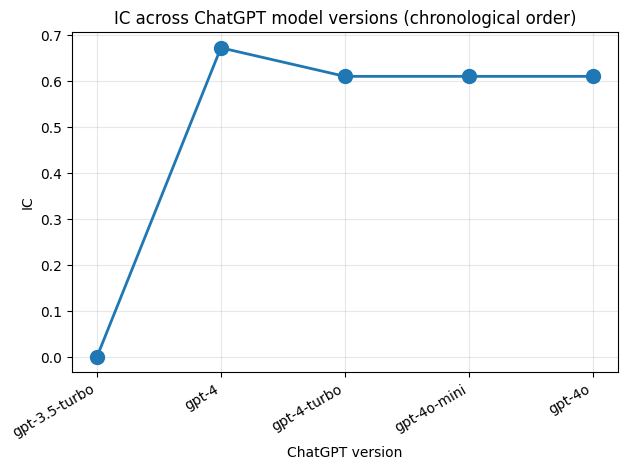
\includegraphics[width=0.48\textwidth]{../figures/chatgpt_ic_chronological.png}
  \hfill
  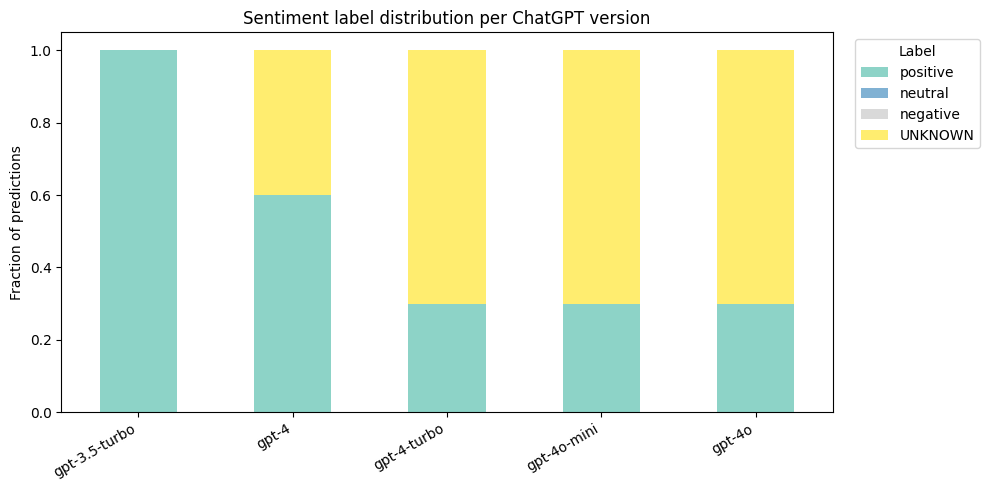
\includegraphics[width=0.48\textwidth]{../figures/llama_ic_base_instruct.png}
  \caption{Left: IC across ChatGPT versions (chronological). Right: IC for Llama~3.2 Base vs.\ Instruct.}
  \label{fig:results}
\end{figure*}

\section{Discussion and Conclusion}

Our results show that political bias in LLMs is not static. For ChatGPT, IC rises sharply with gpt-4 and then plateaus; the shift from all-positive to large UNKNOWN shares may reflect different refusal or classification behavior while still yielding high inconsistency. For Llama, instruction tuning reduces IC for the 1B and 11B vision models but not for 3B; sentiment distributions change markedly with alignment and size. Cross-family, ChatGPT has higher IC and different label patterns than Llama, underscoring that bias is family- and alignment-dependent.

\textbf{Limitations.} We evaluate two families and a fixed set of versions; results may not generalize. IC captures prediction inconsistency under entity substitution but not other dimensions of bias (e.g., framing or ideological stance). The high share of UNKNOWN for some ChatGPT versions complicates interpretation. Differences in API behavior and model access may confound cross-model comparison.

\textbf{Future work.} Extend to more families, longer time horizons, and other bias metrics; relate IC to fairness and stance measures.

\section*{Acknowledgments}
We thank Prof. Adrian Popescu (Fairness in AI, Université Paris-Saclay) and the TEMPO-BIAS project.

\bibliography{custom}

\end{document}
